\documentclass[a4paper,10pt]{article}
\usepackage[T1]{fontenc}
\usepackage{lmodern}
\usepackage{microtype}
\usepackage[a4paper,margin=1.6cm,top=1.5cm,bottom=1.6cm]{geometry}
\usepackage{xcolor}
\usepackage{tikz}
\usetikzlibrary{arrows.meta,positioning,calc}
\usepackage[most]{tcolorbox}
\usepackage{tabularx,booktabs,array}
\usepackage{enumitem}
\usepackage{titlesec}
\usepackage{fancyhdr}
\usepackage[hidelinks]{hyperref}

\definecolor{accent}{HTML}{1F5F7A}
\definecolor{soft}{HTML}{EAF2F5}
\definecolor{muted}{HTML}{5A6670}

\setlength{\parindent}{0pt}
\setlength{\parskip}{3pt}
\setlist{nosep,leftmargin=1.1em,topsep=1pt}
\renewcommand{\arraystretch}{1.15}

\titleformat{\section}{\sffamily\bfseries\large\color{accent}}{}{0pt}{}
\titlespacing*{\section}{0pt}{9pt}{4pt}
\titleformat{\subsection}{\sffamily\bfseries\normalsize\color{accent}}{}{0pt}{}
\titlespacing*{\subsection}{0pt}{6pt}{3pt}

\pagestyle{fancy}
\fancyhf{}
\renewcommand{\headrulewidth}{0pt}
\fancyfoot[L]{\sffamily\footnotesize\color{muted}Exam prep --- user guide}
\fancyfoot[R]{\sffamily\footnotesize\color{muted}\thepage}

\newcommand{\cmd}[1]{\texttt{\bfseries #1}}
\newcommand{\argx}[1]{\texttt{\color{accent}#1}}

\newtcolorbox{card}[1]{enhanced,colback=white,colframe=accent,
  boxrule=0.6pt,arc=2pt,left=6pt,right=6pt,top=4pt,bottom=4pt,
  colbacktitle=accent,coltitle=white,fonttitle=\ttfamily\bfseries,
  title={#1},before skip=5pt,after skip=5pt}
\newtcolorbox{note}{enhanced,colback=soft,colframe=soft,arc=2pt,
  left=6pt,right=6pt,top=4pt,bottom=4pt,before skip=5pt,after skip=5pt}

\begin{document}

{\sffamily
{\LARGE\bfseries\color{accent} Exam prep: how to use it}\par\vspace{2pt}
{\color{muted} Practice sets in the style of your real finals, graded from photos of your work,
each one aimed at what went wrong in the last.}\par}
\vspace{6pt}

\section{The loop}

\begin{center}
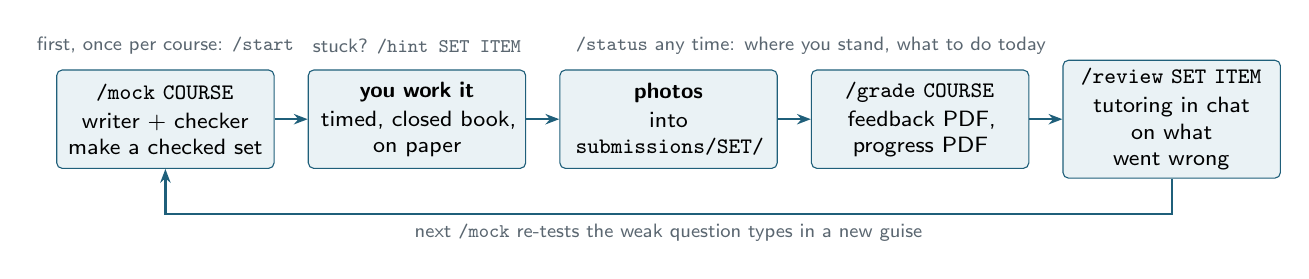
\begin{tikzpicture}[
  box/.style={draw=accent,fill=soft,rounded corners=2pt,align=center,
    font=\sffamily\footnotesize,minimum height=1.25cm,text width=2.55cm,inner sep=3pt},
  arr/.style={-{Stealth[length=5pt]},thick,accent},
  node distance=0.42cm]
  \node[box] (m) {\cmd{/mock COURSE}\\[1pt] writer + checker\\make a checked set};
  \node[box,right=of m] (w) {\textbf{you work it}\\[1pt] timed, closed book,\\on paper};
  \node[box,right=of w] (p) {\textbf{photos}\\[1pt] into\\\texttt{submissions/SET/}};
  \node[box,right=of p] (g) {\cmd{/grade COURSE}\\[1pt] feedback PDF,\\progress PDF};
  \node[box,right=of g] (r) {\cmd{/review SET ITEM}\\[1pt] tutoring in chat\\on what went wrong};
  \draw[arr] (m)--(w); \draw[arr] (w)--(p); \draw[arr] (p)--(g); \draw[arr] (g)--(r);
  \draw[arr] (r.south) -- ++(0,-0.45) -| node[pos=0.25,below,font=\sffamily\scriptsize,text=muted]
    {next \cmd{/mock} re-tests the weak question types in a new guise} (m.south);
  \node[font=\sffamily\scriptsize,text=muted,above=2pt of m.north]
    {first, once per course: \cmd{/start}};
  \node[font=\sffamily\scriptsize,text=muted,above=2pt of g.north west,anchor=south]
    {\cmd{/status} any time: where you stand, what to do today};
  \node[font=\sffamily\scriptsize,text=muted,above=2pt of w.north]
    {stuck? \cmd{/hint SET ITEM}};
\end{tikzpicture}
\end{center}

\argx{COURSE} is the short key you gave the course in \cmd{/start} (\texttt{MATH}, say);
\texttt{courses.md} lists them. Plain requests work too: ``make the next MATH set'', ``the
photos of MATH-T01 are in'', ``how am I doing?'', ``give me a lesson on line integrals''.

\section{Getting started}

\textbf{1. Install} what the project needs (Python with sympy, TeX Live, ImageMagick,
poppler, git): \texttt{SETUP.md}, about 20 minutes, mostly waiting. On Windows the
project runs inside WSL, the Linux built into Windows. \texttt{python3 tools/doctor.py}
checks everything and says what is missing.

\textbf{2. Set up the desktop app} (Code tab):

\begin{tabularx}{\linewidth}{@{}>{\bfseries}l >{\raggedright\arraybackslash}X@{}}
\toprule
Permissions & \emph{Bypass permissions} in the mode selector of this folder, after allowing it
  under Settings $\rightarrow$ Claude Code. Every command runs scripts and agents; without it you
  approve dozens of steps per set. Claude then acts without asking, so keep it to this project.
  \emph{Auto} mode is the cautious alternative. \\
Model & Opus for the main session: it plans and hands the work to cheaper agents. \\
Notifications & On. Writing a set takes 10--30 minutes, grading 5--10. \\
Windows & Start sessions in the \emph{WSL} environment (Ubuntu). Your files: in Explorer at
  \texttt{\textbackslash\textbackslash wsl.localhost\textbackslash Ubuntu\textbackslash home\textbackslash\dots};
  pin that folder. \\
Sessions & A new session for each task (a set, a grading, a review). Long threads re-read
  their history on every message. \\
\bottomrule
\end{tabularx}

\textbf{3. Type \cmd{/start}.} It checks the installation, asks per course for the name,
the date of the final, the other parts of the grade (midterm, homework, lab) and the pass
rules, and your study days. Then it tells you where to put the course's files,
\texttt{<course>/materials/}, most useful first:

\begin{note}
\begin{itemize}
  \item \textbf{past exams}, as many as you can find, each with its answers or solutions
    (three or more make a good course; with fewer, sets match the real exam less well);
  \item the \textbf{study guide} with the exam rules, and the \textbf{lecture schedule} with dates;
  \item the \textbf{formula sheet} allowed in the exam;
  \item \textbf{lecture notes}, slides or book chapters in scope, and \textbf{exercise sets} with solutions;
  \item for a Mathematica part: the course's notebooks.
\end{itemize}
Any file names, any sub-folders. Tell \cmd{/start} which past exams you have already worked.
\end{note}

It then builds the course, one agent at a time: it sorts your files, proposes one real
final to \textbf{hold out} unseen (you decide), transcribes the other exams into a question
bank, writes the syllabus and formula sheet, collects course exercises for topics the old
exams miss, and analyses everything into a \textbf{blueprint}: the question types of your
exam, their weights, how they vary, and where students lose points. Finally it works out
the grade your final must reach, and writes a day plan into \texttt{courses.md}. Building a
course costs roughly one 5-hour usage window on a Pro plan; it stops and resumes cleanly,
so run \cmd{/start} again to continue. Then \cmd{/mock COURSE} makes the first, diagnostic set.

\section{The six commands}

\begin{card}{/start [add|new-quarter]}
Set-up, explained above. Run it again at any time: it continues where it stopped.
\argx{add} adds a course; \argx{new-quarter} moves the old courses to \texttt{archive/} (nothing is
deleted) and sets up the new ones.
\end{card}

\begin{card}{/mock COURSE [diagnostic|train|full|holdout] [MINUTES]}
Makes the next practice set and sends you \texttt{exam.pdf}. The key stays hidden until the set is graded.
\begin{itemize}
  \item \argx{diagnostic}: every question type once, at exam level. \argx{train}: a targeted
    set on your weakest types. \argx{full}: a complete mock in the real exam's format and
    time. \argx{holdout}: the reserved real final (benchmark, plan day only or on request).
  \item No kind given: \texttt{diagnostic} if nothing is graded yet, otherwise today's
    entry in the plan, otherwise \texttt{train}.
  \item \argx{MINUTES}: time budget, training sets only, default 90.
  \item If an earlier set is still ungraded, it asks you to grade or drop it first.
    Say so if you will sit the set on a later day, so topics not yet lectured are judged for that day.
\end{itemize}
{\small\color{muted} Examples: \texttt{/mock MATH} \quad \texttt{/mock MATH train 60} \quad \texttt{/mock MATH full}}
\end{card}

\begin{card}{/hint [SET] ITEM}
While you work a set: the smallest hint that gets you started on one item, never the solution.
\begin{itemize}
  \item It first asks what you have so far. Then one rung per ask: \textbf{nudge} (a question pointing
    at what in the problem gives the approach away), \textbf{method} (named, and why it applies),
    \textbf{set-up} (the first step written down, not worked out). Nothing more until it is graded: no
    answers, no checking your result.
  \item Every hint is logged in \texttt{submissions/SET/hints.json}. On paper: a circled \textbf{H}
    where you continue, and pause the timer while you chat.
  \item At grading, work above the H scores as usual. What the hint gave and the lines built on it score
    nothing, and you also see what the answer would have scored with the hint allowed.
  \item The next training set brings that question type back \emph{first}, with the same move behind a
    different cue. \texttt{progress.pdf} lists each hint and how the re-test went.
  \item Training sets mainly. On a diagnostic or full mock it warns first; none on the held-out exam.
\end{itemize}
{\small\color{muted} Examples: \texttt{/hint MATH-T01 5.2} \quad \texttt{/hint 3.1} (the set you are working on)}
\end{card}

\begin{card}{/grade COURSE [SET]}
Grades your handed-in set, records the scores and rebuilds the progress report.
\begin{itemize}
  \item \argx{SET}: default is the newest set without feedback.
  \item Before you run it, put photos of every page, in order, in
    \texttt{<course>/submissions/SET/} (jpg, png, heic, webp or pdf). Multiple-choice letters,
    time spent and skipped items go in \texttt{answers.txt} there or in chat.
    Mathematica work goes in as the \texttt{.nb} file. Photos still in Downloads? Say so; it copies them.
  \item It reports the page count. Check it, because a missing page is graded as blank.
  \item You get the feedback PDF, the key PDF and \texttt{progress.pdf}. In chat: the score and
    grade equivalent, the top two or three fixes, any readings to double-check, and the items worth a \cmd{/review}.
  \item Think a reading or deduction is wrong? Say which item and why. It gets regraded, and the old rows are replaced.
  \item It never starts the next set. That waits for your \cmd{/mock}.
\end{itemize}
{\small\color{muted} Examples: \texttt{/grade MATH} \quad \texttt{/grade MATH MATH-D01}}
\end{card}

\begin{card}{/review SET ITEM}
A tutoring thread on one graded question: what you wrote, where and why it went wrong, how to do it right.
\begin{itemize}
  \item \texttt{/review MATH-D01 3.2}. With only \argx{SET}, or \texttt{latest}, it lists the items and
    suggests the ones that lost the most points. Loose names work too (``the flux one'').
  \item It opens with a diagnosis: the line where it went wrong, the misunderstanding behind it,
    and the right first move. Then you choose \textbf{guided} (hints, you write each step) or
    \textbf{explained} (the full solution, with checks you can use in the exam).
  \item Ask follow-ups in the same thread. It ends with you stating the method in your own words,
    a redo from a blank page, and a fresh variant to try.
  \item Ask for a \textbf{video} (``animate it'') and you get a 1--2 minute clip: your own lines
    appear one by one, the wrong term is boxed with the reason, then it rewinds to your last good
    line and continues correctly (saved in \texttt{<course>/animations/}). Every line is numbered:
    ask ``why line 12?'' and the answer comes in chat. Needs the optional video packages.
  \item If a whole question type is missing, it offers a \textbf{lesson} PDF (saved in \texttt{<course>/lessons/}).
    Scores are never changed here.
\end{itemize}
\end{card}

\begin{card}{/status}
Rebuilds and sends \texttt{progress/progress.pdf}. For each course it gives the days and study
days left, the sets done, the grade figures (with the share of the exam they are measured on)
and any ungraded set. It also says what to do today: the earliest exam first, then the weakest
heavy question types.
\end{card}

\section{Handing in: the conventions}

\begin{note}
\begin{itemize}
  \item \textbf{Timed and closed book}, with only the aids on the cover. Otherwise the score means nothing.
  \item Items marked \emph{not yet lectured}: write \texttt{SKIP}. They are not counted.
  \item \textbf{Stuck before you can start?} Use \cmd{/hint}: write a circled H where you continue, pause
    the timer. The log tells the grader the rest.
  \item \textbf{Hint from an AI tutor elsewhere?} Draw a thick black bar in the margin next to the lines
    written with help, and say what the hint was about. Those lines score nothing, and that
    question type will not move up a level.
  \item \textbf{Time stamps} (elapsed time) under each problem. An answer that is correct but took
    more than 1.5 times its budget does not move up a level either.
  \item \textbf{Photos in page order, into the folder}, not pasted into the chat (the grader cannot see
    pasted images, and the main session pays to read them). \texttt{prep\_photos.sh} sorts them by
    capture time, then by file name, rotates and shrinks them into \texttt{pages/}, and never
    touches the originals.
\end{itemize}
\end{note}

\section{Ground rules}

\begin{note}
\begin{itemize}
  \item Sets are written \textbf{only on your command} (\cmd{/mock}). Grading never starts one.
  \item No set reaches you before the checker passes it, and no key before your work is graded.
  \item One real final per course is \textbf{held out} in \texttt{<course>/holdout/}: no agent that
    writes or checks sets ever opens it, and you sit it as \texttt{-H01} in the last week for an honest benchmark.
  \item Scores come only from the grader's JSON via \texttt{ledger.py record}, never from editing by hand.
  \item One agent at a time, earliest exam first, to stay under the usage limit.
  \item Your files, work and grades stay on your computer, and git ignores them.
\end{itemize}
\end{note}

\section{Where things are}

\begin{tabularx}{\linewidth}{@{}>{\ttfamily}l X@{}}
\toprule
courses.md & your courses, exam dates, held-out exams, banked grades and the day plan \\
<course>/materials/ & the files you dropped in; \texttt{intake.json} says what each one is \\
<course>/holdout/ & the reserved real final, unseen until you sit it \\
<course>/bank/ & the past exams, transcribed; \texttt{blueprint.md} next to it is the analysis \\
<course>/sets/SET/ & \texttt{exam.pdf}, \texttt{key.pdf}, \texttt{spec.json} (why these items), \texttt{set.json}, \texttt{check/} (checker's verdict) \\
<course>/submissions/SET/ & your photos, \texttt{answers.txt}, notebooks, \texttt{hints.json} (from \cmd{/hint}); \texttt{pages/} is generated \\
<course>/feedback/SET.pdf & the grader's feedback for that set \\
<course>/lessons/ & lesson PDFs, one per question type you asked about \\
<course>/ledger.jsonl & every graded item ever: the source for all statistics \\
progress/progress.pdf & the one progress report for all courses \\
archive/ & the courses of earlier quarters \\
\bottomrule
\end{tabularx}

\smallskip
\textbf{Set ids:} \texttt{MATH-D01} diagnostic, \texttt{-T01, -T02, \dots} training,
\texttt{-F01} full mock, \texttt{-H01} held-out real exam.

\section{Under the hood}

\begin{tabularx}{\linewidth}{@{}>{\bfseries}l >{\itshape}l X@{}}
\toprule
Step & Who & What happens \\
\midrule
Set-up & Sonnet agents, Opus & \texttt{intake.md} sorts your files, \texttt{transcribe.md} turns each past exam
  into the \emph{bank}, \texttt{syllabus.md}, \texttt{seeds.md} and \texttt{toolkit.md} write the course facts,
  conventions and extra exercises, and an Opus agent writes the \emph{blueprint} (\texttt{blueprint.md}).
  \texttt{course.py} keeps track of the steps. \\
Spec   & \texttt{ledger.py next} & Picks the question types (``archetypes''), levels, points and minutes from your ledger. No AI involved. \\
Write  & Opus agent & \texttt{prompts/writer.md}: writes the set and key from the spec, the blueprint and
  the bank, avoiding variations you have already seen. \\
Check  & Sonnet agent & \texttt{prompts/checker.md}: solves the set \emph{blind}, then compares with the key. If it says \texttt{FIX NEEDED}, the writer fixes the set (at most two rounds), and an item that still fails is dropped. \texttt{ledger.py checkset} then validates the files. \\
Grade  & Sonnet agent & \texttt{prompts/grader.md}: transcribes your handwriting, grades against the rubric, tags the first error, and writes feedback as \texttt{.json} and \texttt{.pdf}. \\
Record & \texttt{ledger.py record} & Validates the grader's JSON into \texttt{ledger.jsonl}, the only source of scores. \texttt{build\_report.py} then writes \texttt{progress.pdf}. \\
Hint   & \texttt{hints.py} & Loads one item of a set you are working (question, earlier hints, and the key for the tutor's eyes only) and logs each hint. \texttt{ledger.py record} refuses feedback that credits work done after a logged hint. \\
Review & \texttt{item\_context.py} & Loads one item (question, your work, grading, key, pitfalls) into chat. \texttt{select\_review.py} ranks the items worth reviewing. For a video the session writes a storyboard (\texttt{prompts/storyboard.md}) and \texttt{animate.sh} renders it with Manim. \\
Extras & Sonnet agents & \texttt{lesson.md}: a mini-course on one archetype. \texttt{holdout.md}: turns the reserved real exam into a gradable set without changing it. \\
\bottomrule
\end{tabularx}

\smallskip
The chat session is only the \emph{orchestrator}. It runs scripts and passes files between agents,
and never reads exam PDFs, photos or keys itself. That keeps each session cheap and long-lived.

\section{How the next set adapts to you}

\begin{itemize}[leftmargin=1.1em]
  \item \textbf{Mastery} per question type is a recency-weighted average, where each older attempt
    counts half as much. Each attempt adds the evidence $\min(1,\ \text{score fraction}\times c)$,
    with $c = 0.65,\ 1.0,\ 1.1$ for levels 1, 2, 3. Skipped items are ignored and blanks count as 0.
  \item \textbf{Status:} \emph{exam-ready} ($\geq 0.80$ and last tried at level $\geq 2$),
    \emph{close} ($\geq 0.55$), \emph{needs-work}, \emph{unmeasured}.
  \item \textbf{Next level} for a question type: $\geq 80\%$ goes one level up, unless you had help
    or took more than 1.5 times the budget. 50--80\% stays the same. Below 50\% goes one level down,
    except after help when the rest of the answer was right ($\geq 80\%$ with the help allowed): then it stays.
  \item \textbf{Training sets} rank the lectured question types by
    weight $\times$ (1 $-$ mastery), $\times 1.5$ if the last attempt was below 50\%, plus a small
    bonus for staleness, and fill the minute budget from the top. They also add one
    \emph{retention check} on an exam-ready type you have not seen for 5 or more days. Types you
    needed a \cmd{/hint} for last time come first. The writer sees your recent errors on each type,
    and for a hint what you had to be told and what should have cued it.
  \item \textbf{Grade figures} (out of 10): \emph{on measured part} is the grade over the types tried so far;
    \emph{coverage} is the share of the exam's weight that has been measured; \emph{banked} counts untried types as 0, a lower bound.
    The pass line in the report is the grade your final must reach, given your other components.
  \item \textbf{Error tags:} concept, method, setup, algebra, sign, arithmetic, notation,
    justification, misread, incomplete. ``Where the points go'' in \texttt{progress.pdf} totals them.
\end{itemize}

\newpage
\section{What it costs}

Claude plans meter usage per 5-hour window and per week, in percent, not dollars. To
compare tasks, the table gives the \emph{API-equivalent}: the tokens priced at list rates
(Opus \$4 in / \$20 out, Sonnet \$2 / \$10 per million tokens; re-reading cached context
\$0.20, writing it 1.25$\times$ the input price). \textbf{Fresh} tokens are new input plus
output; \textbf{re-read} tokens are the context a model sends again on every step, at 5--10\%
of the fresh rate.

\begin{tabularx}{\linewidth}{@{}>{\ttfamily}l l r r r r@{}}
\toprule
\normalfont Function & Who works & Fresh & Re-read & \$ & of a Pro 5\,h window \\
\midrule
/start, one course\,$^*$ & Sonnet agents, Opus blueprint & 1--2M & 15--30M & 15--30 & 60--120\% \\
/mock train       & Opus writer, Sonnet checker & 0.8M & 8M   & 6.7     & 26\% \\
/mock diagnostic  & same                        & 0.9--1.7M & 11--23M & 8--14 & 31--54\% \\
/mock full\,$^*$  & same, larger set            & $\sim$1.2M & $\sim$12M & 10--16 & 38--62\% \\
holdout prep\,$^*$& Sonnet                      & $\sim$0.3M & $\sim$4M & 1--3 & 4--12\% \\
/grade            & Sonnet grader, chat         & 0.3M & 2.2M & 1.3--1.5 & 5--6\% \\
/hint, one item\,$^*$ & chat session           & $\sim$20k & $\sim$0.4M & 0.2--0.5 & 1--2\% \\
/review, 10 turns\,$^*$ & chat session          & $\sim$0.2M & $\sim$3M & 1--1.5 & 4--6\% \\
\quad + video\,$^*$ & storyboard, render is free & $\sim$30k & $\sim$0.5M & +0.5 & +2\% \\
lesson            & Sonnet                      & 0.16M & 4.8M & 1.7     & 7\% \\
/status\,$^*$     & scripts, one turn           & $<$20k & 0.3M & 0.1--0.3 & $<$1\% \\
one chat message  & warm cache                  & $\sim$3k & 0.1M & 0.03--0.10 & 0.1--0.4\% \\
new session, 1st message & cache is written     & 0.11M & --- & 0.3--0.6 & 1--2\% \\
\bottomrule
\end{tabularx}

{\small\color{muted} Rows without $^*$ were measured on real runs in October 2026; rows with $^*$
are estimates from the nearest measured run. The last column uses one calibration on a Pro
plan: about \$26 API-equivalent filled a 5-hour window and about \$200 a week ($\pm$30\%; Anthropic
does not publish the limits). Max plans have several times more.}

\begin{itemize}[leftmargin=1.1em]
  \item \textbf{The 5-hour window is the one that bites.} On Pro, about three training sets or two
    full mocks fill it. Writing a set is $\sim$60\% of the cost of a loop, so space the writing out
    over the day, and set up one course per window.
  \item \textbf{A heavy study day} (two training sets, four gradings, eight reviews) is $\sim$\$29
    API-equivalent: about one Pro window.
  \item \textbf{Cheaper chat:} a review thread on Sonnet costs half per message. Start a new session
    for a new task.
  \item \textbf{Extra usage} (credits), if you turn it on, bills work past a limit at API rates, so the
    dollar column is roughly what you would pay for the part that overflows.
  \item \textbf{Calibrate for your plan:} note the app's usage meters before and after a task and
    compare with \texttt{python3 tools/usage\_report.py}, which shows what this project used per day
    and model. Chats outside this project use the same limits and are not counted there.
\end{itemize}

\section{By hand, if you want}

\begin{tcolorbox}[enhanced,colback=white,colframe=muted!40,boxrule=0.4pt,arc=2pt,left=6pt,top=3pt,bottom=3pt]
\small\ttfamily
python3 tools/doctor.py \hfill{\normalfont\color{muted} is everything installed?}\\
python3 tools/course.py list \hfill{\normalfont\color{muted} courses and how far their set-up is}\\
python3 tools/course.py state MATH \hfill{\normalfont\color{muted} the set-up steps of one course}\\
python3 tools/ledger.py status \hfill{\normalfont\color{muted} all courses at a glance}\\
python3 tools/ledger.py mastery MATH \hfill{\normalfont\color{muted} mastery table for one course}\\
python3 tools/ledger.py next MATH -{}-kind train -{}-minutes 60 \hfill{\normalfont\color{muted} preview what a set would target}\\
python3 tools/build\_report.py \hfill{\normalfont\color{muted} rebuild progress.pdf}\\
python3 tools/item\_context.py MATH-D01 \hfill{\normalfont\color{muted} list a set's items and scores}\\
python3 tools/hints.py show MATH-T01 \hfill{\normalfont\color{muted} the hints logged for a set}\\
python3 tools/usage\_report.py \hfill{\normalfont\color{muted} what this project used, per day and model}
\end{tcolorbox}

\end{document}
